\documentclass[letterpaper]{article}

% used for enumerating problem parts by letter
\usepackage{enumerate}
% used for margins
\usepackage[letterpaper,left=1.25in,right=1.25in,top=1in,bottom=1in]{geometry}
% used for header and page numbers
\usepackage{fancyhdr}
% used for preventing paragraph indentation
\usepackage[parfill]{parskip}
% used for subsection indentation
\usepackage{changepage}
% used for inserting images
\usepackage{graphicx}
% used for eps graphics
\usepackage{epstopdf}
\usepackage{amssymb}
% used for links
%\usepackage{hyperref}


\pagestyle{fancy}
\fancyfoot{}
% header/footer settings
\lhead{Kevin Nash (kjn33)}
\chead{EECS 325 -- Project 4}
\rhead{\today}
\cfoot{\thepage}

\begin{document}

\section*{CANVAS}

% stuff here?

\subsection*{The Application Protocol}

My protocol, \textbf{C}oloring \textbf{AN}d \textbf{V}iewing \textbf{A}rt
\textbf{S}quares, provides a simple means of changing the ``pixels'' of a
single common ``image.'' In reality the image is an array of text and its
pixels are Full Block (\texttt{U+2588}) characters. Message passing is handled
by UDP over POSIX sockets. Clients send instructions to the server, and in
response the server modifies or erases a pixel in the image. Clients can
also request the current state of the image, as well as a sample image.

The idea of having an indefinite number of clients modify an image
simultaneously was partially inspired by the Reddit's April Fools Day gag for
2017, /r/place.

(https://redditblog.com/2017/04/18/place-part-two)

\subsection*{Running Client and Server}

First ensure that the executables are ready to run by compiling/cleaning
with \texttt{make}.

To run the server, simply invoke \texttt{./proj4d port}, where \texttt{port} is
the port number that is available for you to use on your system.

To run a client, simply invoke \texttt{./proj4 host port}, where \texttt{host}
is the host name of the server you wish to reach (e.g.
\texttt{localhost}, \texttt{eecslab-5.case.edu}) and \texttt{port} is the port
number that the server is expecting connections on.

\subsection*{Protocol Commands}

\textit{Note: All commands are case-sensitive. In general all capitals should be used.}

\textbf{MARK}\quad Marks (colors or recolors) a certain pixel in the image. 

\begin{adjustwidth}{2em}{0em}
    Format: MARK X Y COLOR\\
    Parameters:
    \begin{adjustwidth}{1em}{0em}
    \begin{tabular}{ l l }
        X & the x-coordinate of the pixel\\
        Y & the y-coordinate of the pixel\\
        COLOR & the color that replaces the pixel's current color\\
        & [ RED $\vert$ GRN $\vert$ YEL $\vert$ BLU $\vert$ MAG $\vert$ CYN $\vert$ WHT ]
    \end{tabular}
    \end{adjustwidth}
\end{adjustwidth}

\textbf{ERAS}\quad Erases a certain pixel in the image.

\begin{adjustwidth}{2em}{0em}
    Format: ERAS X Y\\
    Parameters:
    \begin{adjustwidth}{1em}{0em}
    \begin{tabular}{ l l }
        X & the x-coordinate of the pixel\\
        Y & the y-coordinate of the pixel
    \end{tabular}
    \end{adjustwidth}
\end{adjustwidth}

\textbf{PRNT}\quad Prints the current image.

\begin{adjustwidth}{2em}{0em}
    Format: PRNT\\
    Parameters:
    \begin{adjustwidth}{1em}{0em}
    none
    \end{adjustwidth}
\end{adjustwidth}

\textbf{TEST}\quad Prints a sample image for testing display compatibility.

\begin{adjustwidth}{2em}{0em}
    Format: TEST\\
    Parameters:
    \begin{adjustwidth}{1em}{0em}
    none
    \end{adjustwidth}
\end{adjustwidth}

\textbf{TIME}\quad Prints the current server time.

\begin{adjustwidth}{2em}{0em}
    Format: TIME\\
    Parameters:
    \begin{adjustwidth}{1em}{0em}
    none
    \end{adjustwidth}
\end{adjustwidth}

\subsection*{Justifications}

UDP was selected for use instead of TCP due to the nature of the application
compared with UDP's strengths. CANVAS does not require a persistent connection,
messages are short and the data transfer is minimal. Additionally, the server
does not need to retain information about clients after it gives a response.

\subsection*{How Things Should Look}

The sample image, requested with TEST, on the programmer's machine and on eecslab-5.

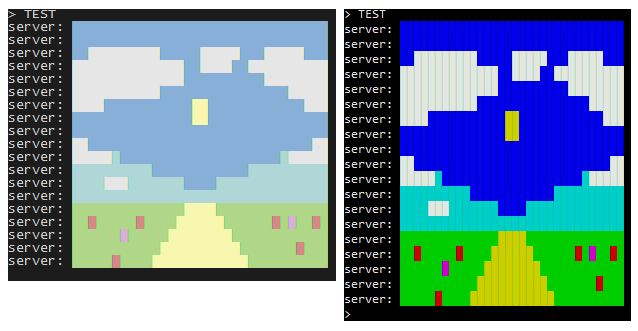
\includegraphics[scale=0.9]{test.png}

\end{document}
